
\documentclass[xetex,professionalfont]{beamer}

\usepackage{amsmath}

\usepackage{mathtools}

\usepackage{amssymb}

\usepackage{xspace}

\usepackage{booktabs}


\usepackage{fontspec}
\setmonofont[Scale=0.7]{Droid Sans Mono} %

\usepackage[caption=false]{subfig}
\captionsetup{belowskip=0pt,aboveskip=0pt}

\usepackage{csquotes}

\usepackage{copyrightbox}

\usepackage[english]{babel}


\usepackage{tikz}

\usepackage{pgfplots}

\usetikzlibrary{backgrounds,arrows,automata}

\definecolor{xblue}{RGB}{210,224,255}
\definecolor{xyellow}{RGB}{255,255,205}
\definecolor{xred}{RGB}{255,205,205}
\definecolor{xgreen}{RGB}{205,255,205}


\hypersetup{pdftitle={DLVC Lecture 7},pdfsubject={},pdfauthor={Christopher Pramerdorfer},colorlinks,urlcolor=tuwcvl_cvl_blue,linkcolor=tuwcvl_textlight,citecolor=tuwcvl_textlight}

\makeatletter\renewcommand{\CRB@setcopyrightfont}{\tiny\color{lightgray}}

\let\oldemph\emph
\renewcommand\emph[1]{\textcolor{tuwcvl_cvl_blue}{#1}}

\usefonttheme[onlymath]{serif}

\usetheme{dlvc}


\definecolor{dred}{rgb}{0.85,0,0.1}
\definecolor{dgreen}{rgb}{0,0.85,0.1}
\definecolor{dblue}{rgb}{0,0.1,0.85}


\newcommand{\ie}{\mbox{i.e.}\xspace} %
\newcommand{\eg}{\mbox{e.g.}\xspace} %

\DeclareMathOperator*{\argmin}{arg\,min}
\DeclareMathOperator*{\argmax}{arg\,max}

\newcommand{\NN}{\mathbb{N}}
\newcommand{\ZZ}{\mathbb{Z}}
\newcommand{\QQ}{\mathbb{Q}}
\newcommand{\RR}{\mathbb{R}}

\renewcommand{\vec}[1]{\ensuremath{\mathbf{#1}}}

\newcommand{\va}{\vec{a}}
\newcommand{\vb}{\vec{b}}
\newcommand{\vc}{\vec{c}}
\newcommand{\ve}{\vec{e}}
\newcommand{\vr}{\vec{r}}
\newcommand{\vs}{\vec{s}}
\newcommand{\vt}{\vec{t}}
\newcommand{\vu}{\vec{u}}
\newcommand{\vv}{\vec{v}}
\newcommand{\vw}{\vec{w}}
\newcommand{\vx}{\vec{x}}
\newcommand{\vy}{\vec{y}}
\newcommand{\vz}{\vec{z}}
\newcommand{\vo}{\vec{o}}
\newcommand{\vm}{\vec{m}}
\newcommand{\vn}{\vec{n}}

\makeatletter
\let\@@magyar@captionfix\relax
\makeatother

\newcommand{\vA}{\vec{A}}
\newcommand{\vW}{\vec{W}}
\newcommand{\vX}{\vec{X}}
\newcommand{\bth}{\boldsymbol{\theta}}
\newcommand{\cD}{\mathcal{D}}
\newcommand{\cB}{\mathcal{B}}

\DeclareMathOperator*{\sgn}{sgn}
\DeclareMathOperator*{\mean}{mean}
\DeclareMathOperator*{\iou}{iou}
\DeclareMathOperator*{\ap}{AP}
\DeclareMathOperator*{\map}{mAP}

\makeatletter
\def\verbatim@font{\linespread{1}\normalfont\ttfamily}
\makeatother


\title{Deep Learning for Visual Computing}
\subtitle{Object Detection}
\author{Christopher Pramerdorfer}
\institute{Computer Vision Lab, TU Wien}

\begin{document}


\begin{frame}
	\maketitle
\end{frame}


\begin{frame}
	\frametitle{Topics}

	Beyond image classification

	\bigskip

	Object detection
	\begin{itemize}
		\item Introduction \& performance metrics
	\end{itemize}

	\bigskip

	Deep object detection
	\begin{itemize}
		\item Sliding window approach
		\item Two-stage detectors (R-CNN)
		\item One-stage detectors (YOLO)
		\item Feature pyramid networks
	\end{itemize}

\end{frame}


\begin{frame}
	\frametitle{Beyond Image Classification}

	We have focused on image classification
	\begin{itemize}
		\item Fundamental computer vision task
		\item We now know how to achieve good performance
	\end{itemize}

	\bigskip

	Rest of lecture will focus on more challenging tasks

\end{frame}


\begin{frame}
	\frametitle{Beyond Image Classification}

	Recall our ingredients for image classification
	\begin{itemize}
		\item A suitable dataset
		\item A network with a suitable final layer (linear layer)
		\item A suitable loss function $L(\bth)$ (cross-entropy)
		\item An algorithm for computing $\nabla L(\bth)$ (backpropagation)
		\item An algorithm for updating $\bth$ on this basis (Adam)
		\item An intuitive performance metric (accuracy)
	\end{itemize}

\end{frame}


\begin{frame}
	\frametitle{Beyond Image Classification}

	These ingredients are universal

	\bigskip

	Steps 4 and 5 are not task-specific and can be reused

	\bigskip

	So when tackling a new problem, ask yourself
	\begin{itemize}
		\item Do I have enough (labeled) data? %
		\item What is a suitable network output? %
		\item What is a suitable loss function? %
		\item What is a good metric for evaluation?
	\end{itemize}

\end{frame}


\begin{frame}
	\frametitle{Beyond Image Classification}

	Answer to first question is almost always \enquote{no}
	\begin{itemize}
		\item Networks are usually pre-trained on ImageNet
		\item First learn what different objects look like
		\item Then adapt for other tasks (transfer learning)
	\end{itemize}
	\bigskip

	\bigskip

	PyTorch provides such models directly
	\begin{itemize}
		\item \texttt{net = models.resnet34(pretrained=True)}
	\end{itemize}

\end{frame}


{
\setbeamertemplate{footline}{}
\begin{frame}

	\begin{tikzpicture}[remember picture,overlay]
		\fill[white] (current page.north west) rectangle (current page.south east);
	\end{tikzpicture}

	\begin{center}
		\textcolor[rgb]{0.9,0.9,0.9}{blank page}
	\end{center}

\end{frame}
}


\begin{frame}
	\frametitle{Object Detection}
	\framesubtitle{Task Definition}

	Given an image and $C$ class labels (\eg \{bird, cat, dog\})
	\begin{itemize}
		\item Draw bounding boxes around all instances of all classes
		\item Assign correct class label to each bounding box
	\end{itemize}

	\smallskip

	\begin{center}
		\copyrightbox[b]
		{\includegraphics[width=6.5cm]{images/pets}}
		{\centering Image adapted from 123rf.com}
	\end{center}

\end{frame}


\begin{frame}
	\frametitle{Object Detection}
	\framesubtitle{Challenges \& Opportunities}

	More challenging than image classification
	\begin{itemize}
		\item Same basic challenges (see lecture 1)
		\item More complex task
		\item Harder to implement efficiently
	\end{itemize}

	\bigskip

	Many useful applications such as
	\begin{itemize}
		\item Face detection (\eg surveillance)
		\item Autonomous driving (\eg road sign detection)
	\end{itemize}

\end{frame}


\begin{frame}
	\frametitle{Object Detection}
	\framesubtitle{Datasets}

	COCO is the most popular dataset with detection labels

	\bigskip

	\begin{center}
		\copyrightbox[b]
		{\includegraphics[width=8cm]{images/coco.jpg}}
		{\centering Image from \href{http://cocodataset.org}{cocodataset.org}}
	\end{center}

\end{frame}


\begin{frame}
	\frametitle{Object Detection}
	\framesubtitle{Progress}

	\begin{center}
		\copyrightbox[b]
		{\includegraphics[width=9cm]{images/coco-performance}}
		{\centering Image from \href{https://paperswithcode.com/sota/object-detection-on-coco}{paperswithcode.com}}
	\end{center}

\end{frame}


\begin{frame}
	\frametitle{Object Detection}
	\framesubtitle{Detector Output}

	What is a suitable object detector output?

	\bigskip

	Most detectors predict the following
	\begin{itemize}
		\item $N$ bounding boxes $\cB_n$
		\item $N$ corresponding class labels $c_n$
		\item $N$ corresponding confidence scores $p_n$
	\end{itemize}

\end{frame}


\begin{frame}
	\frametitle{Object Detection}
	\framesubtitle{Loss Function}

	Two tasks at once
	\begin{itemize}
		\item Predict accurate bounding boxes (regression)
		\item Assign them correct class labels (classification)
	\end{itemize}

	\bigskip

	We thus usually have $L(\bth)=L_{\text{loc}}(\bth)+L_{\text{clf}}(\bth)$
	\begin{itemize}
		\item First term measures bounding box accuracy (e.g. L1 loss)
		\item Second term is classification loss (e.g.~cross-entropy loss)
	\end{itemize}

\end{frame}


\begin{frame}
	\frametitle{Object Detection}
	\framesubtitle{Performance Metrics}

	\emph{Intersection over union} (\emph{IoU}) base measure

	\bigskip

	\begin{center}
		\copyrightbox[b]{\includegraphics[width=4.5cm]{images/iou}}
		{\centering Image from Wikipedia}
	\end{center}

\end{frame}


\begin{frame}
	\frametitle{Object Detection}
	\framesubtitle{Performance Metrics}

	Ignoring class labels and given a
	\begin{itemize}
		\item Single ground-truth bounding box $\cB'$
		\item Single predicted bounding box $\cB$
		\item IoU threshold $t_{iou}$
	\end{itemize}

	\bigskip

	$\cB$ is a
	\begin{itemize}
		\item \emph{True positive} (\emph{TP}) if $\iou(\cB',\cB)\geq t_{iou}$
		\item \emph{False positive} (\emph{FP}) otherwise
	\end{itemize}

	\bigskip

	In second case there is also one \emph{false negative} (\emph{FN})
	\begin{itemize}
		\item No $\cB$ with sufficient IoU with $\cB'$
	\end{itemize}

\end{frame}


\begin{frame}
	\frametitle{Object Detection}
	\framesubtitle{Performance Metrics}

	Ignoring class labels and given multiple bounding boxes
	\begin{itemize}
		\item \emph{Precision} = TPs / (TPs + FPs)
		\item \emph{Recall} = TPs / (TPs + FNs)
	\end{itemize}

	\bigskip

	In case of multiple $\cB$ for a given $\cB'$ %
	\begin{itemize}
		\item Count $\cB$ with highest $p$ as TP, others als FPs
	\end{itemize}

	\bigskip

	Both metrics are in $[0,1]$
	\begin{itemize}
		\item Ideally precision $=$ recall $=1$
	\end{itemize}

\end{frame}


\begin{frame}
	\frametitle{Object Detection}
	\framesubtitle{Performance Metrics}

	Use confidence threshold $t_p$ to balance recall vs.~precision

	\bigskip

	Increasing $t_p$ results in fewer detections
	\begin{itemize}
		\item Usually increases precision %
		\item Usually decreases recall %
	\end{itemize}

\end{frame}


\begin{frame}
	\frametitle{Object Detection}
	\framesubtitle{Performance Metrics}

	\emph{Precision vs.~recall curves} highlight this behavior
	\begin{itemize}
		\item Plotting precision and recall over $t_p\in[0,1]$
		\item Area under curve is called \emph{average precision} (AP)
	\end{itemize}

	\smallskip

	\begin{center}
		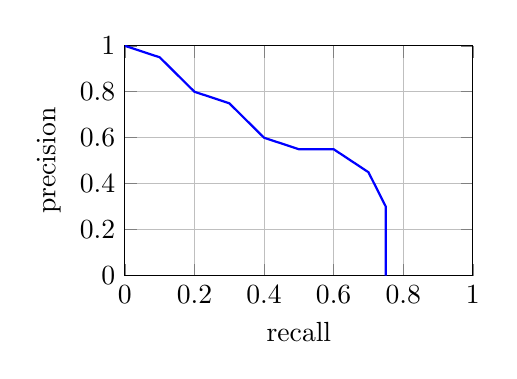
\begin{tikzpicture}
			\begin{axis}[width=6cm,height=4.5cm,xlabel=recall,ylabel=precision,xmin=0,xmax=1,ymin=0,ymax=1,grid]
				\addplot[thick,blue] coordinates {
						(0,1)
						(0.1,0.95)
						(0.2,0.8)
						(0.3,0.75)
						(0.4,0.6)
						(0.5,0.55)
						(0.6,0.55)
						(0.7,0.45)
						(0.75,0.3)
						(0.75,0)
					};
			\end{axis}
		\end{tikzpicture}
	\end{center}

\end{frame}


\begin{frame}
	\frametitle{Object Detection}
	\framesubtitle{Performance Metrics}

	AP is most popular base metric
	\begin{itemize}
		\item Concise measure of detector performance
		\item For single $t_{iou}$ and single class
	\end{itemize}

	\bigskip

	\emph{Mean average precision} (mAP) extends this to $C$ classes
	\[
		\text{mAP}_{t_{iou}}=\frac{1}{C}\sum_c^C\text{AP}_c
	\]

\end{frame}


\begin{frame}
	\frametitle{Object Detection}
	\framesubtitle{Performance Metrics}

	And further to multiple $t_{iou}$, \eg
	\[
		\text{mAP}=\frac{1}{10}(\text{mAP}_{0.50}+\cdots+\text{mAP}_{0.95})
	\]

	\bigskip

	Confusingly mAP is sometimes named just AP in papers
	\begin{itemize}
		\item Like in COCO performance chart above
	\end{itemize}

\end{frame}


{
\setbeamertemplate{footline}{}
\begin{frame}

	\begin{tikzpicture}[remember picture,overlay]
		\fill[white] (current page.north west) rectangle (current page.south east);
	\end{tikzpicture}

	\begin{center}
		\textcolor[rgb]{0.9,0.9,0.9}{blank page}
	\end{center}

\end{frame}
}


\begin{frame}
	\frametitle{Deep Object Detection}

	Many interesting approaches and methods exist
	\begin{itemize}
		\item See survey papers such as [1] for an overview
	\end{itemize}

	\bigskip
	Virtually all use a classification network as \emph{backbone}
	\begin{itemize}
		\item Transfer learning as mentioned earlier
	\end{itemize}

	\bigskip
	We will cover three approaches
	\begin{itemize}
		\item Naive sliding window approach %
		\item Two-stage detectors (R-CNN)
		\item Single-stage detectors (YOLO)
	\end{itemize}

\end{frame}


\begin{frame}
	\frametitle{Deep Object Detection}
	\framesubtitle{Sliding Window Approach}

	Training
	\begin{itemize}
		\item Train a classifier for $C+1$ classes %
		\item Additional \enquote{background} class %
	\end{itemize}

	\bigskip

	Detection
	\begin{itemize}
		\item Slide fixed-size window over image
		\item Predict class-scores for every window
		\item Perform non-maximum suppression %
	\end{itemize}

\end{frame}


\begin{frame}
	\frametitle{Deep Object Detection}
	\framesubtitle{Sliding Window Approach}

	\begin{center}
		\copyrightbox[b] {
			\begin{tikzpicture}
				\node [inner sep=0pt,above right]{\includegraphics[width=6.5cm]{images/face-detection}};
				\draw[thick,green,opacity=0.2] (0.5,1.5) rectangle (1.5,2.55);
				\draw[thick,green,opacity=0.4] (0.7,1.5) rectangle (1.7,2.55);
				\draw[thick,green,opacity=0.6] (0.9,1.5) rectangle (1.9,2.55);
				\draw[thick,green,opacity=0.8] (1.1,1.5) rectangle (2.1,2.55);
				\draw[thick,green] (1.3,1.5) rectangle (2.4,2.55);
			\end{tikzpicture}
		}
		{\centering Image adapted from apple.com}
	\end{center}

\end{frame}


\begin{frame}
	\frametitle{Deep Object Detection}
	\framesubtitle{Sliding Window Approach}

	Inefficient
	\begin{itemize}
		\item Many windows to classify %
	\end{itemize}

	\bigskip

	Single fixed-size window (no scale invariance) %
	\begin{itemize}
		\item Must process image at multiple scales (more inefficient)
		\item Inaccurate bounding boxes (fixed aspect ratio) %
	\end{itemize}

	\bigskip

	Cannot handle multiple objects in same window (softmax) %

\end{frame}


\begin{frame}
	\frametitle{Deep Object Detection}
	\framesubtitle{Two-Stage Detectors}

	Improve efficiency by
	\begin{itemize}
		\item First generating many \emph{region proposals} %
		\item Classifying these proposals
	\end{itemize}

	\medskip

	\begin{center}
		\copyrightbox[b]{\includegraphics[width=8cm]{images/r-cnn}}
		{\centering Image adapted from [1]}
	\end{center}

\end{frame}


\begin{frame}
	\frametitle{Deep Object Detection}
	\framesubtitle{Two-Stage Detectors}

	Region proposals have different size and aspect ratio
	\begin{itemize}
		\item Solves window-related problems %
		\item Warp to common size to support minibatch predictions
	\end{itemize}

	\medskip

	\begin{center}
		\copyrightbox[b]{\includegraphics[width=8cm]{images/r-cnn}}
		{\centering Image adapted from [1]}
	\end{center}

\end{frame}


\begin{frame}
	\frametitle{Deep Object Detection}
	\framesubtitle{Two-Stage Detectors}

	Approach of \emph{R-CNN}
	\begin{itemize}
		\item First successful deep-learning-based object detector
		\item Clunky design and training, see [2] if interested
	\end{itemize}

	\medskip

	\begin{center}
		\copyrightbox[b]{\includegraphics[width=8cm]{images/r-cnn}}
		{\centering Image adapted from [1]}
	\end{center}

\end{frame}


\begin{frame}
	\frametitle{Deep Object Detection}
	\framesubtitle{Two-Stage Detectors}

	Approach still inefficient
	\begin{itemize}
		\item Got to classify many region proposals
	\end{itemize}

	\bigskip

	More efficient extension
	\begin{itemize}
		\item Process complete (high-resolution) image once
		\item Project region proposals onto suitable conv layer output %
		\item Classify each resulting feature map region
	\end{itemize}

\end{frame}


\begin{frame}
	\frametitle{Deep Object Detection}
	\framesubtitle{Two-Stage Detectors}

	Approach was introduced by \emph{Fast R-CNN} [3]


	\bigskip

	\begin{center}
		\copyrightbox[b]{\includegraphics[width=10cm]{images/fast-rcnn}}
		{\centering Image adapted from [1]}
	\end{center}

\end{frame}


\begin{frame}
	\frametitle{Deep Object Detection}
	\framesubtitle{Two-Stage Detectors}

	Region proposal step remains a bottleneck
	\begin{itemize}
		\item Generic algorithms (\eg selective search [4])
		\item Not integrated into network
		\item Usually quite slow
	\end{itemize}

	\medskip

	\begin{center}
		\copyrightbox[b]{\includegraphics[width=9cm]{images/selective-search}}
		{\centering Image adapted from [4]}
	\end{center}

\end{frame}


\begin{frame}
	\frametitle{Deep Object Detection}
	\framesubtitle{Two-Stage Detectors}

	There are improvements that address this
	\begin{itemize}
		\item Faster R-CNN is an example
	\end{itemize}

	\bigskip
	R-CNN variants are \emph{two-stage detectors}
	\begin{itemize}
		\item First generate $r$ region proposals
		\item Then analyze these proposals
	\end{itemize}

	\bigskip
	Modern detectors are \emph{one-stage detectors}
	\begin{itemize}
		\item Combine both stages, inference time independent of $r$
	\end{itemize}

\end{frame}


\begin{frame}
	\frametitle{Deep Object Detection}
	\framesubtitle{One-Stage Detectors}

	Most one-stage detectors utilize \emph{anchor boxes}
	\begin{itemize}
		\item Fixed set of reference bounding boxes
		\item At different scales and aspect ratios
	\end{itemize}

	\bigskip

	\begin{center}
		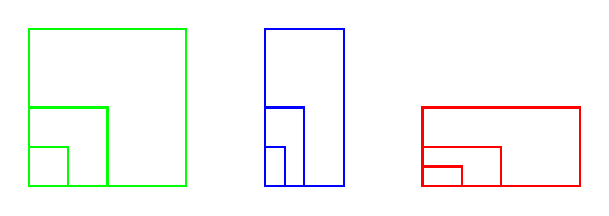
\begin{tikzpicture}
			\draw[thick,green,scale=0.5] (0,0) rectangle (1,1);
			\draw[thick,green,scale=1.0] (0,0) rectangle (1,1);
			\draw[thick,green,scale=2.0] (0,0) rectangle (1,1);

			\draw[thick,blue,scale=0.5,xshift=6cm] (0,0) rectangle (0.5,1);
			\draw[thick,blue,scale=1.0,xshift=3cm] (0,0) rectangle (0.5,1);
			\draw[thick,blue,scale=2.0,xshift=1.5cm] (0,0) rectangle (0.5,1);

			\draw[thick,red,scale=0.5,xshift=10cm] (0,0) rectangle (1,0.5);
			\draw[thick,red,scale=1.0,xshift=5cm] (0,0) rectangle (1,0.5);
			\draw[thick,red,scale=2.0,xshift=2.5cm] (0,0) rectangle (1,0.5);
		\end{tikzpicture}
	\end{center}

\end{frame}


\begin{frame}
	\frametitle{Deep Object Detection}
	\framesubtitle{One-Stage Detectors}

	\emph{YOLO} is a popular anchor-based detector familiy
	\begin{itemize}
		\item High detection performance
		\item Runs in real-time
	\end{itemize}

	\bigskip

	Many versions exist
	\begin{itemize}
		\item We will cover v2, and v3
		\item Overall approach (detector head) identical
	\end{itemize}

\end{frame}


\begin{frame}
	\frametitle{Deep Object Detection}
	\framesubtitle{YOLO}

	Simplified overall approach
	\begin{itemize}
		\item Divide input image into coarse $S\times S$ grid
		\item For each grid cell and anchor box, predict class labels (if any)
		\item Perform non-maximum suppression
	\end{itemize}

	\medskip

	\begin{center}
		\copyrightbox[b]
		{\includegraphics[width=10cm]{images/yolo-approach.jpg}}
		{\centering Image from pjreddie.com}
	\end{center}

\end{frame}


\begin{frame}
	\frametitle{Deep Object Detection}
	\framesubtitle{YOLO v2}

	More precisely, given an anchor box we seek to predict
	\begin{itemize}
		\item The IoU overlap $p$ with the most relevant object %
		\item The offset and scale of the box $(x,y,w,h)$ %
		\item $C$ class scores %
	\end{itemize}

	\bigskip

	To constrain the number of detections %
	\begin{itemize}
		\item Divide the image into grid (e.g. $7\times7$)
		\item Align each anchor box with the center of each grid cell
		\item Predict the above for every box and every cell
	\end{itemize}

\end{frame}


\begin{frame}
	\frametitle{Deep Object Detection}
	\framesubtitle{YOLO v2}

	Assuming $k$ anchor boxes and a $7\times7$ grid
	\begin{itemize}
		\item Output is $k\cdot(5+C)\times7\times7$
		\item Can be implemented using conv and pooling layers
	\end{itemize}

	\bigskip

	Backbone pools down to desired grid size
	\begin{itemize}
		\item For instance $224\mapsto112\mapsto56\mapsto28\mapsto14\mapsto7$
	\end{itemize}

	\bigskip

	\emph{Detector head} consists of conv layers only
	\begin{itemize}
		\item Last one has $k\cdot(5+C)$ channels
		\item YOLO v2 uses 4 layers in total (implementation detail)
	\end{itemize}

\end{frame}


\begin{frame}
	\frametitle{Deep Object Detection}
	\framesubtitle{YOLO v2}

	Network has no linear layers
	\begin{itemize}
		\item \emph{Fully convolutional network} (\emph{FCN}) architecture
		\item Supports varying input (image) resolution
	\end{itemize}

\end{frame}


\begin{frame}
	\frametitle{Deep Object Detection}
	\framesubtitle{YOLO v2 -- Training}

	Pretrain backbone, then fine-tune for detection

	\bigskip

	For every training image, grid cell, and bounding box label
	\begin{itemize}
		\item Find the anchor box with the highest IoU
		\item Compute and assign $(p,x,y,h,w,o_1,\dots,o_C)$
		\item Assign $(0,\dots)$ to all unassigned anchor boxes
	\end{itemize}

\end{frame}


\begin{frame}
	\frametitle{Deep Object Detection}
	\framesubtitle{YOLO v2 -- Training}

	Weighted sum of three L2 losses per anchor box
	\begin{itemize}
		\item Confidence loss (loss on $p$)
		\item Classification loss (loss on class scores) *
		\item Localization loss (loss on $x,y,w,h$) *
	\end{itemize}

	\bigskip

	(*) Only if IoU with ground-truth box is sufficient

\end{frame}


\begin{frame}
	\frametitle{Deep Object Detection}
	\framesubtitle{YOLO v2 -- Inference}

	Network always predicts $k\cdot S\cdot S$ detections %
	\begin{itemize}
		\item But most have $p\approx0$
		\item Perform per-class non-maximum suppression %
	\end{itemize}

	\medskip

	\begin{center}
		\copyrightbox[b]
		{\includegraphics[height=3.5cm]{images/yolo-bbs.jpg} \quad \includegraphics[height=3.5cm]{images/yolo-bbs-nms.jpg}}
		{\centering Image adapted from \href{https://www.youtube.com/watch?v=9s_FpMpdYW8}{Youtube}} %
	\end{center}

\end{frame}


\begin{frame}
	\frametitle{Deep Object Detection}
	\framesubtitle{YOLO v2 -- Limitations}

	Issues with
	\begin{itemize}
		\item Small objects
		\item Predicting tight bounding boxes
	\end{itemize}

	\bigskip

	Because backbone feature tensor has low resolution of $S\times S$
	\begin{itemize}
		\item Late in network so semantically strong features
		\item But limited amount of spatial information due to pooling
	\end{itemize}

\end{frame}


\begin{frame}
	\frametitle{Deep Object Detection}
	\framesubtitle{Feature Pyramid Networks}

	Could address this by duplicating detector heads
	\begin{itemize}
		\item Attach to different conv layers
	\end{itemize}

	\bigskip

	\begin{center}
		\copyrightbox[b]
		{\includegraphics[width=4.5cm]{images/feature-pyramid}}
		{\centering Image from [6]}
	\end{center}

\end{frame}


\begin{frame}
	\frametitle{Deep Object Detection}
	\framesubtitle{Feature Pyramid Networks}

	Earlier layers have higher resolution but are semantically weaker
	\begin{itemize}
		\item We want both
	\end{itemize}

	\bigskip

	\begin{center}
		\copyrightbox[b]
		{\includegraphics[width=4.5cm]{images/feature-pyramid}}
		{\centering Image from [6]}
	\end{center}

\end{frame}


\begin{frame}
	\frametitle{Deep Object Detection}
	\framesubtitle{Feature Pyramid Networks}

	\emph{Feature pyramid networks} (\emph{FPNs}) achieve this by combining
	\begin{itemize}
		\item High-resolution but semantically weaker features
		\item Lower-resolution but semantically stronger features
	\end{itemize}

	\bigskip

	\begin{center}
		\copyrightbox[b]
		{\includegraphics[width=10cm]{images/fpn}}
		{\centering Image from [6]}
	\end{center}

\end{frame}



\begin{frame}
	\frametitle{Deep Object Detection}
	\framesubtitle{Feature Pyramid Networks}

	Accomplished by
	\begin{itemize}
		\item Upsampling lower-resolution features
		\item Combining features using sum operation
	\end{itemize}

	\smallskip

	\begin{center}
		\copyrightbox[b]
		{\includegraphics[width=4.5cm]{images/fpn-op}}
		{\centering Image from [6]}
	\end{center}

\end{frame}


\begin{frame}
	\frametitle{Deep Object Detection}
	\framesubtitle{Feature Pyramid Networks}

	Requires matching number of channels
	\begin{itemize}
		\item Fixed number of channels (\eg $256$)
		\item Implemented using pointwise convolutions
	\end{itemize}

	\smallskip

	\begin{center}
		\copyrightbox[b]
		{\includegraphics[width=4.5cm]{images/fpn-op}}
		{\centering Image from [6]}
	\end{center}

\end{frame}


\begin{frame}
	\frametitle{Deep Object Detection}
	\framesubtitle{Feature Pyramid Networks}

	FPNs aggregate and refine features
	\begin{itemize}
		\item Independent of base network architecture and task
	\end{itemize}

	\bigskip

	In object detection context
	\begin{itemize}
		\item FPN (or alternatives) forms the \emph{neck} of the detector
		\item Independent of backbone and head network architectures
	\end{itemize}

\end{frame}


\begin{frame}
	\frametitle{Deep Object Detection}
	\framesubtitle{YOLO v3}

	YOLO v3 uses a FPN neck with 3 scales
	\begin{itemize}
		\item One YOLO head per scale
		\item In addition to other improvements, see [7] if interested
	\end{itemize}

	\bigskip

	\begin{center}
		\copyrightbox[b]
		{\includegraphics[width=10cm]{images/yolo3-arch}}
		{\centering Image adapted from [7]}
	\end{center}

\end{frame}


\begin{frame}
	\frametitle{Deep Object Detection}
	\framesubtitle{YOLO -- Remarks}

	Several improved variants of YOLO exist, such as [8]
	\begin{itemize}
		\item Better backbone network
		\item Improved neck architecture
		\item Better training data augmentation
		\item Overall approach (detector head) largely identical
	\end{itemize}

	\bigskip

	YOLO is a good candidate for object detection
	\begin{itemize}
		\item Modern variants perform well (COCO mAP around 55\%)
		\item Have great speed vs.~performance trade-off
	\end{itemize}

\end{frame}


\begin{frame}
	\frametitle{Deep Object Detection}
	\framesubtitle{YOLO -- Remarks}

	Speed vs.~performance on COCO [8]

	\bigskip

	\begin{center}
		\copyrightbox[b]
		{\includegraphics[width=6cm]{images/yolo-perf}}
		{\centering Image from [8]}
	\end{center}

\end{frame}


\begin{frame}
	\frametitle{Deep Object Detection}
	\framesubtitle{YOLO -- Showcase}

	\begin{center}
		\copyrightbox[b]
		{\includegraphics[width=6.5cm]{images/yolo-vid}}
		{\centering Image from \href{https://www.youtube.com/watch?v=1_SiUOYUoOI}{youtube}}
	\end{center}

\end{frame}

\renewcommand\emph[1]{\oldemph{#1}}

\begin{frame}
	\frametitle{Bibliography}

	[1] Zaidi et al.~\href{https://arxiv.org/abs/2104.11892}{Deep Object Detection Survey}.~2021 \\\medskip
	[2] Girshick et al.~\href{https://arxiv.org/abs/1311.2524}{R-CNN}.~2013 \\\medskip
	[3] Girshick.~\href{https://arxiv.org/abs/1504.08083}{Fast R-CNN}.~2015 \\\medskip
	[4] Uijlings et a.~\href{https://staff.fnwi.uva.nl/th.gevers/pub/GeversIJCV2013.pdf}{Selective Search}.~2013 \\\medskip
	[5] Redmon \& Farhadi.~\href{https://arxiv.org/abs/1612.08242v1}{YOLO v2}.~2016 \\\medskip
	[6] Lin et al.~\href{https://arxiv.org/abs/1612.03144}{Feature Pyramid Networks}.~2017 \\\medskip
	[7] Redmon \& Farhadi.~\href{https://pjreddie.com/media/files/papers/YOLOv3.pdf}{YOLO v3}.~2017 \\\medskip
	[8] Wang et al.~\href{https://arxiv.org/abs/2011.08036v2}{Scaled-YOLO v4}.~2021

\end{frame}


\end{document}
